\sectionframe{Modellierung}

\begin{frame}
 \frametitle{Beispiel: Produktionsproblem (Lewig Sanstetten)}
 \begin{figure}
  \centering
  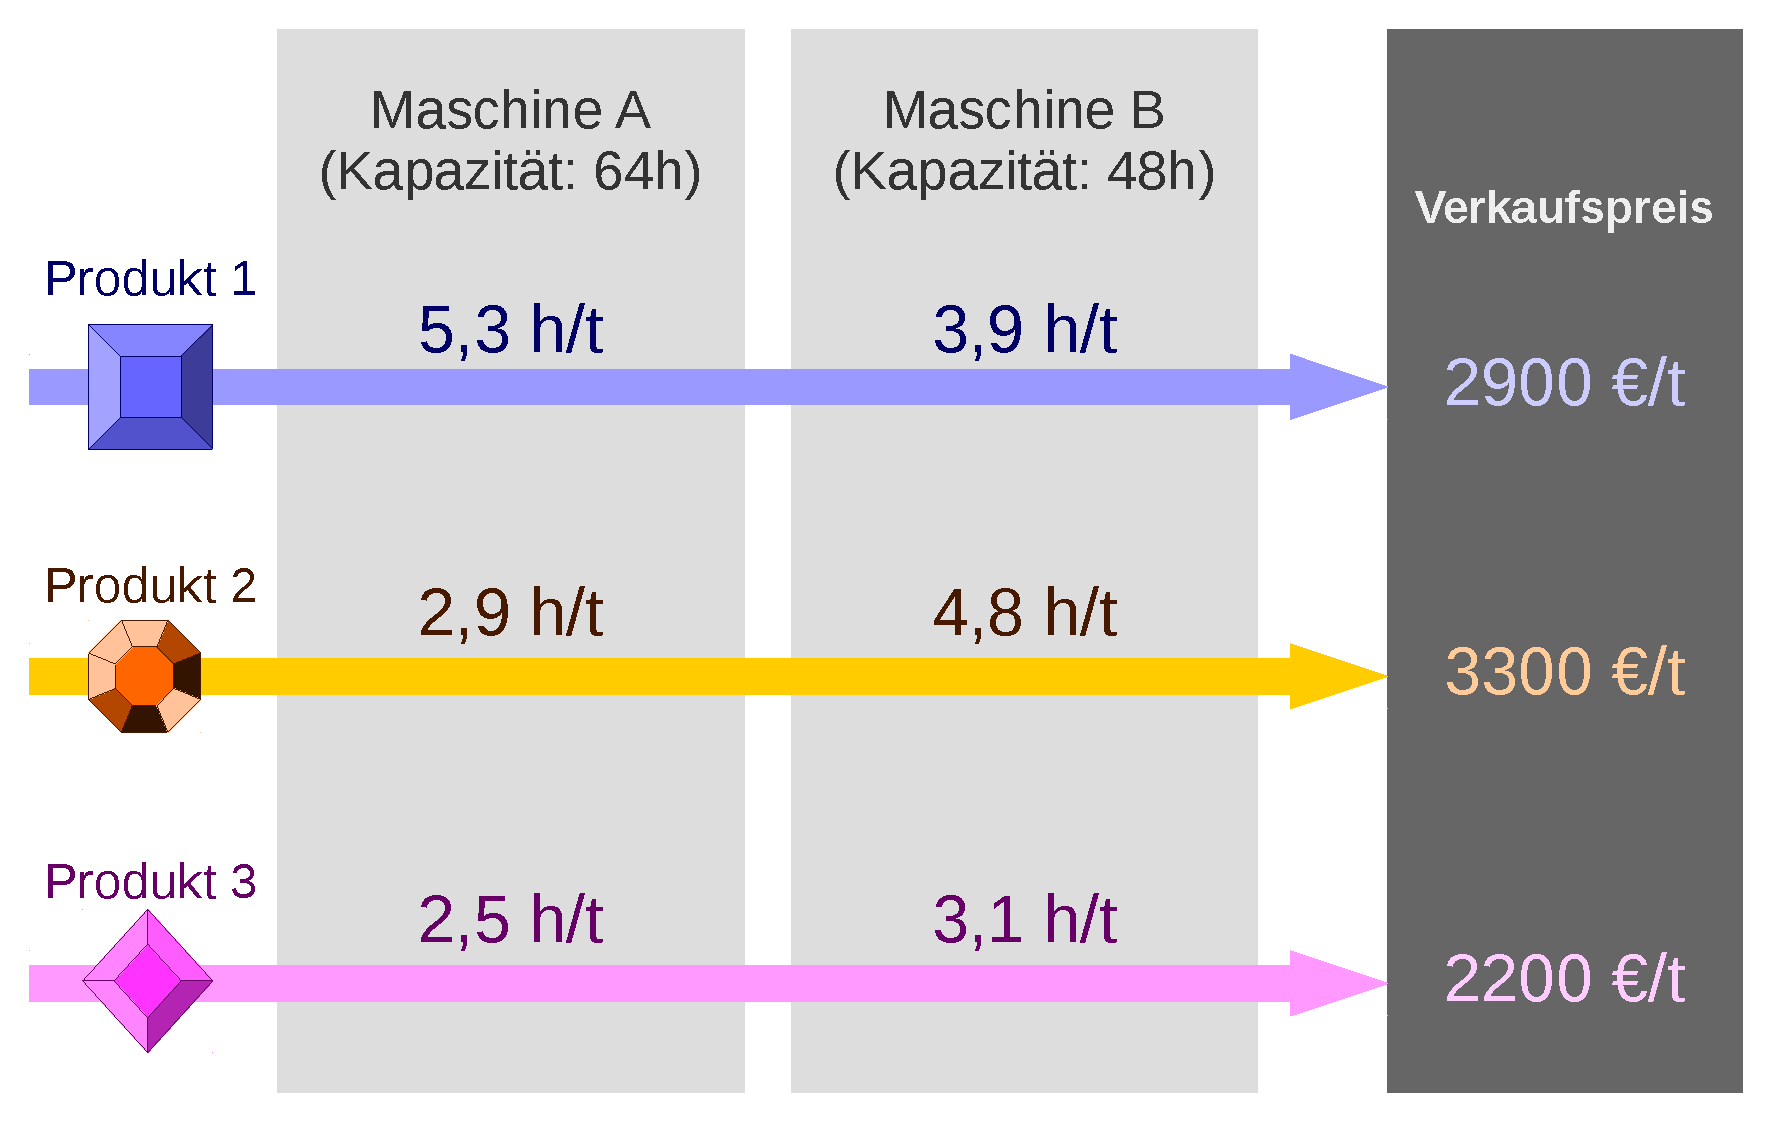
\includegraphics[width=\linewidth]{Bilder/LewigSanstetten}
 \end{figure}
 
 Wie viel soll von jedem Produkt produziert werden?
\end{frame}

\begin{frame}
 \frametitle{Was ist ein Modell?}
 \begin{itemize}
  \item Abstrakte Abbildung eines realen Systems
  \item Zum Beispiel nützlich
  \begin{itemize}
   \item zum Systemdesign
   \item zur Performanceanalyse
   \item \textbf{zur Entscheidungsunterstützung}
  \end{itemize}
  \item Grundsatz: so genau wie nötig, so einfach wie möglich
 \end{itemize}
\end{frame}

\begin{frame}
 \frametitle{Mathematische Optimierungsmodelle zur Entscheidungsunterstützung}
 Bestandteile eines mathematischen Optimierungsmodells\footnote{auch: mathematisches Programm\\\mbox{}}:
 \begin{description}\footnotesize
  \item[Entscheidungsvariablen] Die Größen des Systems, die durch den Entscheider gesetzt werden können
  \begin{itemize}
   \item Im Beispiel: Die Produktionsmengen der Produkte
  \end{itemize}
  \item[Nebenbedingungen] Bedingungen, welche von den Entscheidungsvariablen eingehalten werden müssen um eine sinnvolle Lösung zu erhalten
  \begin{itemize}
   \item Im Beispiel: Die Kapazität der Maschinen
  \end{itemize}  
  \item[Zielfunktion] Eine Funktion der Entscheidungsvariablen, die vom Entscheider optimiert -- d.h. maximiert oder minimiert -- werden soll.
  \begin{itemize}
   \item Im Beispiel: Der Gesamtumsatz
  \end{itemize}  
 \end{description}
\end{frame}

\begin{frame}
 \frametitle{Beispiel: Produktionsproblem -- Entscheidungsvariablen}
 \begin{description}
  \item[$x_1$] Produktionsmenge von Produkt~1
  \item[$x_2$] Produktionsmenge von Produkt~2 
  \item[$x_3$] Produktionsmenge von Produkt~3 
 \end{description}
 
 \begin{block}{Definition: Lösung eines Optimierungsmodells}
  Weisen wir den Entscheidungsvariablen konkrete Werte zu, so heißt dies eine Lösung des Optimierungsmodells. 
 \end{block}
\end{frame}

\begin{frame}
 \frametitle{Beispiel: Produktionsproblem -- Nebenbedingungen}
  
  Kapazität von Maschine A muss eingehalten werden
  \begin{itemize}
   \item $5,3 \cdot x_1 + 2,9 \cdot x_2 + 2,5 \cdot x_3 \leq 64$
  \end{itemize}

  Kapazität von Maschine B muss eingehalten werden
  \begin{itemize}
   \item $3,9 \cdot x_1 + 4,8 \cdot x_2 + 3,1 \cdot x_3 \leq 48$
  \end{itemize}
 
 \begin{block}{Definition: Zulässige Lösungen eines Optimierungsmodells}
  Eine Lösung, welche alle Nebenbedingungen einhält, heißt zulässige Lösung. Die Menge aller zulässigen Lösungen heißt Lösungsraum.
 \end{block}
\end{frame}

\begin{frame}
 \frametitle{Beispiel: Produktionsproblem -- Zielfunktion}
 Maximiere den Umsatz (in k€):
 \begin{itemize}
  \item $\max U(x_1, x_2, x_3) = 2,9\cdot x_1 + 3,3\cdot x_2 + 2,2\cdot x_3$
 \end{itemize}
 
 \begin{block}{Definition: Optimallösung und Optimalwert eines Optimierungsmodells}
  Gibt es eine zulässige Lösung, in der die Zielfunktion ihr Maximum bzw. Minimum über alle zulässigen Lösungen annimmt (was nicht zwingend der Fall sein muss), so ist dies eine Optimallösung und der zugehörige Zielfunktionswert ist der Optimalwert.
 \end{block}
\end{frame}

\begin{frame}\small
 \frametitle{Beispiel: Produktionsproblem -- Vollständiges Optimierungsmodell}
 \begin{tabularx}{\linewidth}{ll@{\quad}>{\itshape\footnotesize}X}
 $\max$ & $2,9\cdot x_1 + 3,3\cdot x_2 + 2,2\cdot x_3$ & (Zielfunktion)\\
 s.t. & $5,3\cdot x_1 + 2,9\cdot x_2 + 2,5\cdot x_3 \leq 64$ & (Nebenbedingung I)\\
      & $3,9\cdot x_1 + 4,8\cdot x_2 + 3,1\cdot x_3 \leq 48$ & (Nebenbedingung II)\\
      & $x_1\geq0,\,x_2\geq0,\,x_3\geq0$ & (Nicht-Negativitäts-Bedingung)\\
\end{tabularx}
\end{frame}




